\documentclass[12pt]{article}
\newif\ifanswer\answertrue%\answerfalse% comment out to show/hide answers
\usepackage{../preamble3}% preamble always after \newif\ifanswer
%\pagenumbering{gobble}
\title{Art Of Problem Solving - AMC 10 \\ Week 3}
\author{Patrick \& James Toche}
\date{June 25, 2021}

\begin{document}
\maketitle
\begin{minipage}{\textwidth}
\begin{abstract}\setlength{\parindent}{0pt}%
Notes on the AMC-10 Course by Art Of Problem Solving (AOPS).
Copyright restrictions may apply. Written for personal use. 
Please report typos and errors over at \url{https://github.com/ptoche/Math/tree/master/aops}. 
\end{abstract}
\end{minipage}

\thispagestyle{empty}
\clearpage


%%%%%%%%%%%%%%%%%%%%%%%%%%%%%%%%%%%%%%%%%%%%%%%%%%%%%%%%%%%%%%%%%%%%%%%%
\subsection*{1.}

\nopagebreak

Consider the set of numbers $\{1, 10, 10^2, 10^3, \dots, 10^{10}\}$. The ratio of the largest element of the set to the sum of the other ten elements of the set is closest to which integer?

\nopagebreak

\fbox{(A) $1$ \quad (B) $9$ \quad (C) $10$ \quad (D) $11$ \quad (E) $101$}

\begin{answer}
The ratio is:
\begin{align*}
\frac{10^{10}}{10^{0}+10^{1}+\ldots+10^{8}+10^{9}}
\end{align*}
The denominator is a geometric sum with ten terms, which may be written in closed-form as
\begin{align*}
10^{0}+10^{1}+\ldots+10^{8}+10^{9}
= 
\frac{1-10^{10}}{1-10\hfill}
=
\frac{10^{10}(10^{-10}-1)}{-9}
=
\frac{10^{10}(1-10^{-10})}{9}
\end{align*}
Plugging this back into the original fraction and simplifying the $10^{10}$ term:
\begin{align*}
\frac{10^{10}}{10^{0}+10^{1}+\ldots+10^{8}+10^{9}}
=
\frac{9}{1-10^{-10}}
\approx
9
\end{align*}
where the $10^{-10}$ term is so small relative to $1$ that it may be neglected
\begin{empheq}[box={\mathbox[colback=white]}]{equation*}
    9
\end{empheq} 
\end{answer}
%%%%%%%%%%%%%%%%%%%%%%%%%%%%%%%%%%%%%%%%%%%%%%%%%%%%%%%%%%%%%%%%%%%%%%%%

\iftoggle{showAnswers}{\newpage}

%%%%%%%%%%%%%%%%%%%%%%%%%%%%%%%%%%%%%%%%%%%%%%%%%%%%%%%%%%%%%%%%%%%%%%%%
\subsection*{2.}

\nopagebreak

For each positive integer $n$, the mean of the first $n$ terms of a sequence is $n$. What is the $2008^{\text{th}}$ term of the sequence?

\nopagebreak

\fbox{(A) $2008$ \quad (B) $4015$ \quad (C) $4016$ \quad (D) $4,030,056$ \quad (E) $4,032,064$}

\begin{answer}
Let $a_{n}$ denote the general term of the sequence and $S_{n}$ its sum:
\begin{align*}
S_{n} = a_{1} + a_{2} + a_{3} + \ldots a_{n}
\end{align*}
The mean of the first $n$ terms is equal to $n$, so:
\begin{align*}
\frac{S_{n}}{n} = n
\implies
S_{n} = n^2
\end{align*}
From the sums sequence we can recover the $a_{n}$ sequence as follows:
\begin{align*}
S_{n+1} - S_{n}
  = a_{n+1}
  = (n+1)^2 - n^2 
  = 2n + 1
\end{align*}
The general term is $a_{n+1}=2n+1$, so we get
\begin{align*}
a_{2008} 
  = 2 \times 2007 + 1 
  = 4015
\end{align*}
\begin{empheq}[box={\mathbox[colback=white]}]{equation*}
    4015
\end{empheq} 
\end{answer}
%%%%%%%%%%%%%%%%%%%%%%%%%%%%%%%%%%%%%%%%%%%%%%%%%%%%%%%%%%%%%%%%%%%%%%%%

\iftoggle{showAnswers}{\newpage}

%%%%%%%%%%%%%%%%%%%%%%%%%%%%%%%%%%%%%%%%%%%%%%%%%%%%%%%%%%%%%%%%%%%%%%%%
\subsection*{3.}

\nopagebreak

On Monday, Millie puts a quart of seeds, $25\%$ of which are millet, into a bird feeder. On each successive day she adds another quart of the same mix of seeds without removing any seeds that are left. Each day the birds eat only $25\%$ of the millet in the feeder, but they eat all of the other seeds. On which day, just after Millie has placed the seeds, will the birds find that more than half the seeds in the feeder are millet?

\nopagebreak

\fbox{(A) Tuesday (B) Wednesday (C) Thursday (D) Friday (E) Saturday}

\begin{answer}
Suppose the millet and the rest of the seeds weigh the same. Each day the amount added to the feeder weighs one unit (one quart). Let $m_{t}$ denote the amount of millet seeds in the bird feeder on day $t$, immediately after refill. Let $a_{t}$ denote the total amount of seeds in the bird feeder on day $t$, immediately after refill. 

The amount of millet seeds evolves according to:
\begin{align*}
m_{1} & = \sfrac{1}{4} \\
m_{2} & = \sfrac{1}{4} +     \left(\sfrac{3}{4}\right) \cdot \left(\sfrac{1}{4}\right) \\
m_{3} & = \sfrac{1}{4} + \left(\sfrac{3}{4}\right)^{2} \cdot \left(\sfrac{1}{4}\right) \\
m_{t} & = \sfrac{1}{4} + \left(\sfrac{3}{4}\right)^{t} \cdot \left(\sfrac{1}{4}\right) 
        = 0.25 + 0.25(0.75)^{t}
\end{align*}

The total amount of seeds (including millet seeds) evolves according to:
\begin{align*}
a_{1} & = 1 \\
a_{2} & = 1 + \left(\sfrac{3}{4}\right)     \cdot \left(\sfrac{1}{4}\right) \\
a_{3} & = 1 + \left(\sfrac{3}{4}\right)^{2} \cdot \left(\sfrac{1}{4}\right) \\
a_{t} & = 1 + \left(\sfrac{3}{4}\right)^{t} \cdot \left(\sfrac{1}{4}\right)
        = 1 + 0.25(0.75)^{t}
\end{align*}

The percentage of millet in the bird feeder immediately after refill must exceed $0.5$:
\begin{align*}
\frac{0.25 + 0.25(0.75)^{t}}{1 + 0.25(0.75)^{t}} 
                             & \geq 0.5 \\
                  (0.75)^{t} & \geq 0.25 \\
\left(\sfrac{3}{4}\right)^{t} & \geq \sfrac{1}{4} \\
\left(\sfrac{4}{3}\right)^{t} & \leq 4
\end{align*}
Now we check some values:
\begin{align*}
\left(\sfrac{4}{3}\right)^{1} \approx 1.333 & < 4 \\
\left(\sfrac{4}{3}\right)^{2} \approx 1.778 & < 4 \\
\left(\sfrac{4}{3}\right)^{3} \approx 2.370 & < 4 \\ 
\left(\sfrac{4}{3}\right)^{4} \approx 3.160 & < 4 \\
\left(\sfrac{4}{3}\right)^{5} \approx 4.214 & > 4 \quad \checkmark
\end{align*}
Thus, $t=5$, which corresponds to Friday. 

\begin{empheq}[box={\mathbox[colback=white]}]{equation*}
    \text{Friday}
\end{empheq} 
\end{answer}
%%%%%%%%%%%%%%%%%%%%%%%%%%%%%%%%%%%%%%%%%%%%%%%%%%%%%%%%%%%%%%%%%%%%%%%%

\iftoggle{showAnswers}{\newpage}

%%%%%%%%%%%%%%%%%%%%%%%%%%%%%%%%%%%%%%%%%%%%%%%%%%%%%%%%%%%%%%%%%%%%%%%%
\subsection*{4.}

\nopagebreak

In the five-sided star shown, the letters $A$, $B$, $C$, $D$, and $E$ are replaced by the numbers $3$, $5$, $6$, $7$, and $9$, although not necessarily in this order. The sums of the numbers at the ends of the line segments $AB$, $BC$, $CD$, $DE$, and $EA$ form an arithmetic sequence, although not necessarily in this order. What is the middle term of the arithmetic sequence?

\nopagebreak

\hfill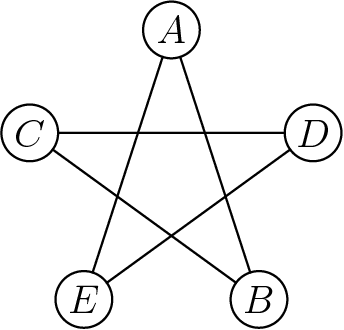
\includegraphics[height=3cm,page=1]{2021-06-25-figure-03}
\vspace{-3ex}

\nopagebreak

\fbox{(A) $9$ \quad (B) $10$ \quad (C) $11$ \quad (D) $12$ \quad (E) $13$}

\begin{answer}
The sums of the numbers at the ends of the line segments are:
\begin{align*}
(A + B) + (B + C) + (C + D) + (D + E) + (E + A) = 2 (A + B + C + D + E)
\end{align*}
Letters $A$, $B$, $C$, $D$, $E$ take values in $\{3,5,6,7,9\}$, so the sum is:
\begin{align*}
2(A + B + C + D + E) = 2(3 + 5 + 6 + 7 + 9) = 2 \cdot 30 = 60
\end{align*}
In an arithmetic sequence, the middle term is equal to the average. Since there are five terms, the average is $60/5=12$.
\begin{empheq}[box={\mathbox[colback=white]}]{equation*}
    \text{middle term}~ = 12
\end{empheq} 
This reasoning does not give an explicit solution, so let's construct the actual solution. To find the solution, note that the common difference $d$ can only be $1$ or $2$. If $d=2$, then the sequence must be $[8,10,12,14,16]$, since $8$ is the lowest possible sum ($3+5$) and $16$ the largest possible sum ($7+9$). But this can be ruled out as follows: all the sums are even, but $6$ is an isolated even integer and therefore cannot be paired with any of the other integers to yield an even sum. This leaves $d=1$ as the only possibility and therefore the values must be one of $[8,9,10,11,12]$, $[9,10,11,12,13]$, $[10,11,12,13,14]$, $[11,12,13,14,15]$, $[12,13,14,15,16]$. Now $6$ is not a problem since these sums contain odd values. Consider our integers and guess what pairing yields the admissible sequence. Here are the pairs and their sum:
\begin{center}
\renewcommand\arraystretch{1}
\begin{tabular}{*{5}{r}}
  (3,5) $\rightarrow$ ~8 & (3,6) $\rightarrow$ ~9 & (3,7) $\rightarrow$ 10 & (3,9) $\rightarrow$ 12 & (5,6) $\rightarrow$ 11 \\
  (5,7) $\rightarrow$ 12 & (5,9) $\rightarrow$ 14 & (6,7) $\rightarrow$ 13 & (6,9) $\rightarrow$ 15 & (7,9) $\rightarrow$ 16 \\
\end{tabular}
\end{center}
Since the sum $13$ cannot be attained with any pair, that leaves $[10,11,12,13,14]$ as the only feasible sequence. And here are the relevant pairs:
\begin{center}
\renewcommand\arraystretch{1}
\begin{tabular}{*{5}{r}}
  10: (3,7) & 11: (5,6) & 12: (3,9) or (5,7) & 13: (6,7) & 14: (5,9) \\
\end{tabular}
\end{center}
Further guesswork yields the star:
\begin{align*}
A = 6 \quad B = 7 \quad C = 3 \quad D = 9 \quad E = 5
\end{align*}
\begin{center}
  \includegraphics[height=3cm,page=2]{2021-06-25-figure-03}
\end{center}
\end{answer}
%%%%%%%%%%%%%%%%%%%%%%%%%%%%%%%%%%%%%%%%%%%%%%%%%%%%%%%%%%%%%%%%%%%%%%%%

\iftoggle{showAnswers}{\newpage}


%%%%%%%%%%%%%%%%%%%%%%%%%%%%%%%%%%%%%%%%%%%%%%%%%%%%%%%%%%%%%%%%%%%%%%%%
\subsection*{5.}

\nopagebreak

In the eight-term sequence $A$, $B$, $C$, $D$, $E$, $F$, $G$, $H$, the value of $C$ is 5 and the sum of any three consecutive terms is 30. What is $A + H$?

\nopagebreak

\fbox{(A) $17$ \quad (B) $18$ \quad (C) $25$ \quad (D) $26$ \quad (E) $43$}

\begin{answer}
We have the following implications:
\begin{align*}
& A + B + C = 30, 
& & C = 5
& & \implies 
B = 25 - A \\
& B + C + D = 30, 
& & B + C = 30 - A
& & \implies 
D = A \\
& C + D + E = 30, 
& & C + D = 5 + A
& & \implies 
E = 25 - A \\
& D + E + F = 30, 
& & D + E = 25
& & \implies 
F = 5 \\
& E + F + G = 30, 
& & E + F = 30 - A
& & \implies 
G = A \\
& F + G + H = 30, 
& & F + G = 5 + A
& & \implies 
H = 25 - A
\end{align*}
The last line implies
\begin{align*}
A + H = 25
\end{align*}
\begin{empheq}[box={\mathbox[colback=white]}]{equation*}
    25
\end{empheq} 
\end{answer}
%%%%%%%%%%%%%%%%%%%%%%%%%%%%%%%%%%%%%%%%%%%%%%%%%%%%%%%%%%%%%%%%%%%%%%%%

\iftoggle{showAnswers}{\newpage}

%%%%%%%%%%%%%%%%%%%%%%%%%%%%%%%%%%%%%%%%%%%%%%%%%%%%%%%%%%%%%%%%%%%%%%%%
\subsection*{6.}

\nopagebreak

Let $a_1$, $a_2$, $\dots$ be a sequence for which $a_1 = 2$, $a_2 = 3$, and $a_n = a_{n - 1}/a_{n - 2}$ for each positive integer $n \ge 3$. What is $a_{2006}$?

\nopagebreak

\fbox{(A) $\dfrac{1}{2}$ \quad (B) $\dfrac{2}{3}$ \quad (C) $\dfrac{3}{2}$ \quad (D) $2$ \quad (E) $3$}

\begin{answer}
Calculating the first few terms  of the sequence:
\begin{align*}
a_{1} & = 2 \\
a_{2} & = 3 \\
a_{3} & = 3/2 \\ 
a_{4} & = 1/2 \\
a_{5} & = 1/3 \\
a_{6} & = 2/3 \\
a_{7} & = 2 \\
a_{8} & = 3
\end{align*}
The sequence repeats every $6$ terms: $a_{7}=a_{1}$, $a_{8}=a_{2}$, \ldots. Since $2004=6\times334$, it follows that $2006$ leaves a remainder of $2$ when divided by $6$. That is $2006 \equiv 2 \bmod{6}$. And thus,
\begin{align*}
 a_{2006} = a_{2}
\end{align*}
\begin{empheq}[box={\mathbox[colback=white]}]{equation*}
    a_{2006} = 3
\end{empheq} 
\end{answer}
%%%%%%%%%%%%%%%%%%%%%%%%%%%%%%%%%%%%%%%%%%%%%%%%%%%%%%%%%%%%%%%%%%%%%%%%

\iftoggle{showAnswers}{\newpage}

%%%%%%%%%%%%%%%%%%%%%%%%%%%%%%%%%%%%%%%%%%%%%%%%%%%%%%%%%%%%%%%%%%%%%%%%
\subsection*{7.}

\nopagebreak

Suppose that $\{a_n\}$ is an arithmetic sequence with $a_1 + a_2 + \dots + a_{100} = 100$ and $a_{101} + a_{102} + \dots + a_{200} = 200$. What is the value of $a_2 - a_1$?

\nopagebreak

\fbox{(A) $0.0001$ \quad (B) $0.001$ \quad (C) $0.01$ \quad (D) $0.1$ \quad (E) $1$}

\begin{answer}
Subtract the two equations:
\begin{align*}
(a_{101} - a_1) + (a_{102} - a_2) + \ldots + (a_{200} - a_{100}) 
= 200 - 100 = 100
\end{align*}
This gives the common difference of every hundred terms repeated one hundred times. Thus the common difference between two terms in the sequence separated by $100$ positions is $1$. The common difference of two sequential terms is one-hundredth of that:
\begin{empheq}[box={\mathbox[colback=white]}]{equation*}
    d = 0.01
\end{empheq}

If you did not see that, perhaps you noticed that the sums satisfy
\begin{align*}
S_{100}  & = 100 \\
S_{200}  & = 300 
\end{align*}
where $S_{200}$ follows by adding the given sums. 
Any arithmetic sum satisfies
\begin{align*}
a_{n} & = a_{1} + (n-1) d \\
S_{n} & = a_{1} + a_{2} + \ldots + a_{n} \\
      & = na_{1} + \left(1 + 2 + \ldots + (n-1)\right)d \\
      & = na_{1} + \frac{(n-1)n}{2} d 
\end{align*}
We thus obtain a linear system of two equations in two unknowns, $a_{1}$ and $d$,
\begin{align*}
S_{100} & = 100a_{1} + \frac{99\cdot100}{2} d  = 100 \\
S_{200} & = 200a_{1} + \frac{199\cdot200}{2} d = 300
\end{align*}
Elimante $a_{1}$ and solve for the common difference $d$
\begin{align*}
\frac{(199-99)\cdot200}{2} d 
  = 300 - 200
  \implies 
d = \dfrac{1}{100}
\end{align*}
\end{answer}
%%%%%%%%%%%%%%%%%%%%%%%%%%%%%%%%%%%%%%%%%%%%%%%%%%%%%%%%%%%%%%%%%%%%%%%%

\iftoggle{showAnswers}{\newpage}

%%%%%%%%%%%%%%%%%%%%%%%%%%%%%%%%%%%%%%%%%%%%%%%%%%%%%%%%%%%%%%%%%%%%%%%%
\subsection*{8.}

\nopagebreak

Let $\{a_k\}$ be a sequence of integers such that $a_1 = 1$ and $a_{m + n} = a_m + a_n + mn$, for all positive integers $m$ and $n$. Then $a_{12}$ is

\nopagebreak

\fbox{(A) $45$ \quad (B) $56$ \quad (C) $67$ \quad (D) $78$ \quad (E) $89$}

\begin{answer}
Let $m=1$. We have $a_{n+1}=1+a_n+n$. The first few terms in the sequence are:
\begin{align*}
  a_{1} & = 1 \\
  a_{2} & = 1 + a_{1} + 1\\
  a_{3} & = 1 + a_{2} + 2\\
 \ldots & \qquad \ldots \\
 a_{12} & = 1 + a_{11} + 11
\end{align*}
Adding up the left- and right-hand sides, all the $a_{n}$ terms cancel out except $a_{12}$:
\begin{align*}
a_{12} & = 12 + (1 + 2 + 3 + \ldots + 11) \\
       & = 12 + \frac{11 \cdot 12}{2} \\
       & = 12 + 66 \\
       & = 78
\end{align*}
\begin{empheq}[box={\mathbox[colback=white]}]{equation*}
    78
\end{empheq} 
\end{answer}
%%%%%%%%%%%%%%%%%%%%%%%%%%%%%%%%%%%%%%%%%%%%%%%%%%%%%%%%%%%%%%%%%%%%%%%%

\iftoggle{showAnswers}{\newpage}

%%%%%%%%%%%%%%%%%%%%%%%%%%%%%%%%%%%%%%%%%%%%%%%%%%%%%%%%%%%%%%%%%%%%%%%%
\subsection*{9.}

\nopagebreak

The first four terms in an arithmetic sequence are $x + y$, $x - y$, $xy$, and $x/y$, in that order. What is the fifth term?

\nopagebreak

\fbox{(A) $-\dfrac{15}{8}$ \quad (B) $-\dfrac{6}{5}$ \quad (C) $0$ \quad (D) $\dfrac{27}{20}$ \quad (E)  $\dfrac{123}{40}$}

\begin{answer}
The difference between consecutive terms, obtained from the first two terms, is $(x-y)-(x+y)=-2y.$ We can also express the third and fourth terms by adding the common difference, which gives the equivalent sequence:
\begin{align*}
& x+y, && x-y, && xy, && x/y \\
& x+y, && x-y, && x-3y, && x-5y
\end{align*}
Equating the third terms gives:
\begin{align*}
     xy & =x-3y \\ 
 x(y-1) & =-3y \\ 
      x & = \frac{-3y}{y-1} 
\end{align*}
Equating the fourth terms and substituting the expression above to eliminate $x$:
\begin{align*}
   \frac{x}{y} & = x-5y \\[1ex]
\frac{-3}{y-1} & = \frac{-3y}{y-1}-5y \\[1ex]
            -3 & = -3y-5y(y-1) \\[1ex]
     5y^2-2y-3 & = 0
\end{align*}
We have a quadratic in $y$, which may be factored as
\begin{align*}
   (5y+3)(y-1) & = 0
\end{align*}

If $y=1$, the sequence would be:
\begin{align*}
x+1, \quad x-1, \quad x, \quad x
\end{align*}
which is not arithmetic. So we reject $y=1$.

The correct solution is the pair:
\begin{align*}
x = -\frac{9}{8}, \quad y = -\frac{3}{5}
\end{align*}

The fifth term in the sequence is therefore
\begin{align*}
\frac{x}{y} - 2y 
  = \frac{-9/8}{-3/5} -2\left(\frac{-3}{5}\right)
  = \frac{45}{24} + \frac{6}{5} 
  = \frac{123}{40}
\end{align*}
\begin{empheq}[box={\mathbox[colback=white]}]{equation*}
    \frac{123}{40}
\end{empheq} 
\end{answer}
%%%%%%%%%%%%%%%%%%%%%%%%%%%%%%%%%%%%%%%%%%%%%%%%%%%%%%%%%%%%%%%%%%%%%%%%

\iftoggle{showAnswers}{\newpage}

%%%%%%%%%%%%%%%%%%%%%%%%%%%%%%%%%%%%%%%%%%%%%%%%%%%%%%%%%%%%%%%%%%%%%%%%
\subsection*{10.}

\nopagebreak

Let $a_1$, $a_2$, $\dots$ be a sequence with the following properties.

(i)  \quad $a_1 = 1$, and

(ii) \quad $a_{2n} = n \cdot a_n$ for any positive integer $n$.

What is the value of $a_{2^{100}}$? (The subscript is $2^{100}$.)

\nopagebreak

\fbox{(A) 1 \quad (B) $2^{99}$ \quad (C) $2^{100}$ \quad (D) $2^{4950}$ \quad (E) $2^{9999}$}

\begin{answer}
Let $n=2^{99}$ and use $a_{2n}=na_{n}$,
\begin{align*}
2^{100} = 2 \times 2^{99} 
\implies
a_{2^{100}} 
  = a_{2 \cdot 2^{99}}
  = 2^{99} a_{2^{99}}
\end{align*}
Applying the same rule repeatedly gives:
\begin{align*}
a_{2^{100}} 
  = 2^{99} 2^{98} a_{2^{98}} 
  = 2^{99} 2^{98} 2^{97} a_{2^{97}} 
  = 2^{99} 2^{98} 2^{97} \ldots 2 a_{2}
\end{align*}
where $a_{2}=a_{1}=1$. So we have
\begin{align*}
a_{2^{100}} 
 & = 2^{99 + 98 + \ldots + 2 + 1} \\
 & = 2^{\frac{99(100)}{2}} \\
 & = 2^{4950}
\end{align*}
\begin{empheq}[box={\mathbox[colback=white]}]{equation*}
    2^{4950}
\end{empheq} 
\end{answer}
%%%%%%%%%%%%%%%%%%%%%%%%%%%%%%%%%%%%%%%%%%%%%%%%%%%%%%%%%%%%%%%%%%%%%%%%


\end{document}
